\documentclass[aspectratio=43,t]{beamer}
%\documentclass[aspectratio=43,t,handout]{beamer}

\usepackage[ansinew]{inputenc}
\usepackage[T1]{fontenc}
%English version FAU Logo
\usepackage[english]{babel}
%German version FAU Logo
%\usepackage[ngerman]{babel}
\usepackage{amsmath,amssymb}
\usepackage{graphicx}
\usepackage{listings}
\usepackage{listings-rust}
\usepackage[backend=biber,sorting=none,doi=true,style=ieee]{biblatex}

% Themes:
%  - fau:          FAU theme
%  - fau-med:      MedFak FAU theme
%  - fau-nat:      NatFak FAU theme
%  - fau-phil:     PhilFak FAU theme
%  - fau-rw:       RWFak FAU theme
%  - fau-rw-jura:  RWFak FB Jura FAU theme
%  - fau-rw-wiso:  RWFak FB WISO FAU theme
%  - fau-tf:       TechFak FAU theme
%
% Options:
%  - image:        Cover image on title page
%  - plain:        Plain title page
%  - longtitle:    Title page layout for long title
\usetheme[longtitle]{fau}

% Enable semi-transparent animation preview
\setbeamercovered{transparent}


\lstset{%
  language=C++,
  tabsize=2,
  basicstyle=\tt\scriptsize,
  keywordstyle=\color{blue},
  commentstyle=\color{green!50!black},
  stringstyle=\color{red},
  numbers=left,
  numbersep=0.5em,
  numberstyle=\tt\tiny
}


\defbibheading{bibliography}{}
\addbibresource[label=primary]{references.bib}
\nocite{*}


% Title, authors, and date
\title[Scalable Molecular Dynamics in AnyDSL]{Scalable AnyDSL Molecular Dynamics application with MPI}
\subtitle{Scaling the Molecular Dynamics implementation in AnyDSL}
\author[Rafael Ravedutti Lucio Machado]{Rafael Ravedutti Lucio Machado}
% English version
\institute[Chair of Computer Science 10]{Chair of Computer Science 10, Friedrich-Alexander University of Erlangen-Nuremberg}
% German version
%\institute[Lehrstuhl f\"ur XYZ]{Lehrstuhl f\"ur XYZ, Friedrich-Alexander-Universit\"at Erlangen-N\"urnberg}
\date{\today}
% Set additional logo (overwrites FAU seal)
%\logo{\includegraphics[width=.15\textwidth]{themefau/art/xxx/xxx.pdf}}


\begin{document}
  % Title
  \maketitle

  { % Motivation
    \setbeamertemplate{footline}{}
    \begin{frame}[noframenumbering]{Motivation}
      Some motivational example\dots
    \end{frame}
  }

  { % Outline
    \setbeamertemplate{footline}{}
    \begin{frame}[noframenumbering]{Outline}
      \tableofcontents
    \end{frame}
  }

  % Body
  \section{AnyDSL}
  \begin{frame}{AnyDSL}
    \begin{block}{Framework for development of domain-specific libraries}
      \begin{itemize}
        \item Higher-order functions
        \item Thorin
        \item Impala
        \item Partial evaluation
      \end{itemize}
    \end{block}
  \end{frame}

  \begin{frame}[fragile]{AnyDSL}
    \begin{lstlisting}[language=Rust]
    fn main() {
      let img = load("dragon.png");
      let blurred = gaussian_blur(img);
    }
    \end{lstlisting}
  \end{frame}

  \begin{frame}[fragile]{AnyDSL}
    \begin{lstlisting}[language=Rust]
    fn gaussian_blur(field: Field) -> Field {
      let stencil: Stencil = { /* ... */ };
      let mut out: Field   = { /* ... */ };

      for x, y in @iterate(out) {
        out.data(x, y) = apply_stencil(x, y, field, stencil);
      }

      out
    }
    \end{lstlisting}
  \end{frame}

  \begin{frame}[fragile]{AnyDSL}
    \begin{lstlisting}[language=Rust]
    fn iterate(field: Field, body: fn(int, int) -> ()) -> () {
      let grid  = (field.cols, field.rows, 1);
      let block = (128, 1, 1);

      with nvvm(grid, block) {
          let x = nvvm_tid_x() + nvvm_ntid_x() * nvvm_ctaid_x();
          let y = nvvm_tid_y() + nvvm_ntid_y() * nvvm_ctaid_y();
          body(x, y);
      }
    }
    \end{lstlisting}
  \end{frame}

  \section{Molecular Dynamics}
  \begin{frame}{Molecular Dynamics}
    \begin{block}{Pair-wise interaction of particles simulation implemented in AnyDSL}
      \begin{itemize}
        \item Cells of particles (bounding boxes)
        \item Neighborlists
        \item Cluster of particles
        \item Target CPU with vectorization instructions and GPU
      \end{itemize}
    \end{block}
  \end{frame}

  \begin{frame}{Molecular Dynamics}
    \begin{block}{Steps}
      \begin{enumerate}
        \item<1-> Initialize grid
        \item<2-> Initialize clusters
        \item<3-> Build neighbor lists
        \item<4-> Compute forces and update particles (for 20 timesteps)
        \item<5-> Redistribute particles and go back to item 2
      \end{enumerate}
    \end{block}
  \end{frame}

  \section{Proposal}
  \begin{frame}{Proposal}
    \begin{block}{Goals}
      \begin{itemize}
        \item Scalable version of the application
        \item First: scale application on homogeneous clusters
        \item In the future: heterogeneous clusters (both CPU and GPU nodes)
        \item Compare scalable implementation with other state-of-the-art versions
      \end{itemize}
    \end{block}
  \end{frame}

  \begin{frame}{Proposal}
    \begin{block}{Steps}
      \begin{itemize}
        \item Domain partitioning
        \item Communication pattern
        \item Synchronization of cells (every timestep)
        \item Particle exchange (after redistribution)
      \end{itemize}
    \end{block}
  \end{frame}

  \begin{frame}{Proposal}
    \begin{block}{Domain partitioning}
      \begin{itemize}
        \item Define configuration of nodes
        \item Split domain accordingly
        \item Define current node bounding box
        \item Include ghost layer cells
        \item \textbf{get\_comm\_time\_steps()}
      \end{itemize}
    \end{block}
  \end{frame}

  \begin{frame}[fragile]{Domain partitioning}
    \begin{lstlisting}[basicstyle=\tiny\ttfamily,language=Rust]
      fn get_node_config(
        world_size: i32,
        rank: i32,
        xcells: i32, 
        ycells: i32, 
        zcells: i32) -> [i32 * 3] { 

        let mut gx = 1, gy = 1, gz = 1; 
        let mut min_missing_factor = xcells * ycells * zcells;

        for i in range(1, world_size) {
          if(world_size % i == 0) { 
            let rem_yz = world_size / i; 

            for j in range(1, rem_yz) {
              if(rem_yz % j == 0) { 
                let k = rem_yz / j; 
                let missing_factor = xcells % i + ycells % j + zcells % k; 

                if(min_missing_factor > missing_factor) {
                  gx = i; 
                  gy = j; 
                  gz = k; 
                  min_missing_factor = missing_factor;
                }
              }
            }    
          }    
        }

        [gx, gy, gz]
      }
    \end{lstlisting}
  \end{frame}

  \begin{frame}[fragile]{Domain partitioning}
    \begin{lstlisting}[basicstyle=\tiny\ttfamily,language=Rust]
    fn @get_comm_rank_bounding_box(
      world_size: i32,
      rank: i32,
      cell_spacing: f64,
      aabb: AABB) -> AABB {

      let mut xmin, xmax, ymin, ymax, zmin, zmax: f64;

      if(world_size > 1) {
        let xcells = math.floor((aabb.max(0) - aabb.min(0)) / cell_spacing) as i32;
        ... /* Analogous to x */

        node_dims = get_node_config(world_size, rank, xcells, ycells, zcells);

        let xlength = (xcells / node_dims(0)) as f64 * cell_spacing;
        ... /* Analogous to x */

        let rank_index = unflat_index(rank, node_dims(0), node_dims(1), node_dims(2));

        xmin = aabb.min(0) + xlength * (rank_index(0) as f64);
        xmax = aabb.min(0) + xlength * ((rank_index(0) + 1) as f64);
        ... /* Analogous to x */

        ... /* Include ghost zone */
      } else {
        ... /* 1 node case */
      }

      AABB {
        min: [xmin, ymin, zmin],
        max: [xmax, ymax, zmax]
      }
    }
    \end{lstlisting}
  \end{frame}

  \begin{frame}[fragile]{Domain partitioning}
    \begin{lstlisting}[basicstyle=\tiny\ttfamily,language=Rust]
    fn @get_comm_rank_bounding_box(
      world_size: i32,
      rank: i32,
      cell_spacing: f64,
      aabb: AABB) -> AABB {

      let mut xmin, xmax, ymin, ymax, zmin, zmax: f64;

      if(world_size > 1) {
        ... /* Bounding box definition */

        if(rank_index(0) > 0) {
          xmin -= (get_comm_time_steps() as f64) * cell_spacing;
        }

        if(rank_index(0) < node_dims(0) - 1) {
          xmax += (get_comm_time_steps() as f64) * cell_spacing;
        } else {
          xmax += cell_spacing;
        }
        ... /* Analogous to x */
      } else {
        ... /* 1 node case */
      }

      AABB {
        min: [xmin, ymin, zmin],
        max: [xmax, ymax, zmax]
      }
    }
    \end{lstlisting}
  \end{frame}

  \begin{frame}{Proposal}
    \begin{block}{Domain partitioning}
      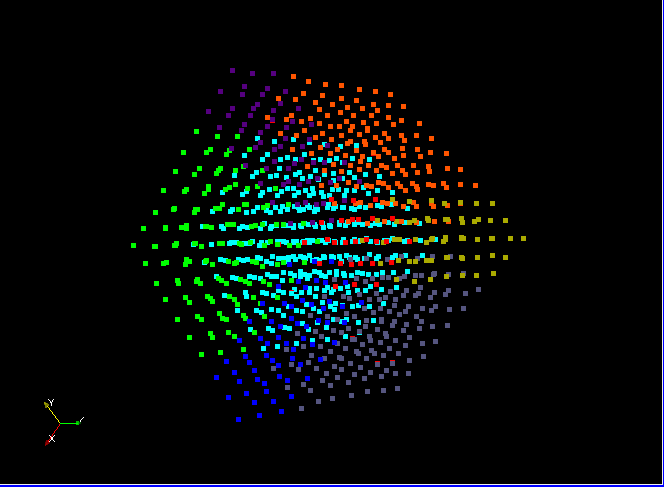
\includegraphics[width=9cm]{domain_partitioning.png}
    \end{block}
  \end{frame}

  \begin{frame}{Proposal}
    \begin{block}{Communication pattern}
      \begin{itemize}
        \item Higher-order function for iteration
        \item Easy to write and change with AnyDSL
      \end{itemize}
    \end{block}
  \end{frame}

  \begin{frame}[fragile]{Communication pattern}
    \begin{lstlisting}[basicstyle=\tiny\ttfamily,language=Rust]
    fn communication_nodes(
      world_size: i32,
      rank: i32,
      grid: Grid,
      body: fn(i32, [i32 * 3], [i32 * 3], [i32 * 3], [i32 * 3]) -> ()) -> () {

      let rank_index = unflat_index(rank, ...);
      let xprev = rank_index(0) > 0;
      let xnext = rank_index(0) < node_dims(0) - 1;
      ...

      if(xnext) {
        @@body(
          flat_index(
            [rank_index(0) + 1, rank_index(1), rank_index(2)],
            node_dims(0), node_dims(1)),
          send_begin1, send_end1, recv_begin1, recv_end1 // for xnext communication
        );     
      }

      if(xprev) {
        @@body(
          flat_index(
            [rank_index(0) - 1, rank_index(1), rank_index(2)],
            node_dims(0), node_dims(1)),
          send_begin2, send_end2, recv_begin2, recv_end2 // for xprev communication
        );     
      }

      ... /* Analogous to x */
    }
    \end{lstlisting}
  \end{frame}

  \begin{frame}{Proposal}
    \begin{block}{Synchronization of cells}
      \begin{itemize}
        \item Update positions, velocity and forces of particles
        \item One-step communication
        \item Every \textbf{get\_comm\_time\_steps()} timesteps
      \end{itemize}
    \end{block}
  \end{frame}

  \begin{frame}[fragile]{Synchronization of cells}
    \begin{lstlisting}[basicstyle=\tiny\ttfamily,language=Rust]
    fn synchronize_ghost_layer_cells(
      grid: &mut Grid,
      accelerator_grid: AcceleratorGrid,
      world_size: i32,
      world_rank: i32) -> () {

      ... /* Transfer data from accelerator to CPU */

      for exchange_rank, send_begin, send_end, recv_begin, recv_end in
          communication_nodes(world_size, world_rank, *grid) {

        pack_ghost_layer_cells(
          mpi_send_buffer, grid, accelerator_grid, send_begin, send_end);

        mpih.irecv(...);
        mpih.send(...);
        mpih.wait(...);

        unpack_ghost_layer_cells(
          mpi_recv_buffer, grid, accelerator_grid, recv_begin, recv_end);
      }

      ... /* Transfer data from CPU to accelerator */
    }
    \end{lstlisting}
  \end{frame}

  \begin{frame}{Proposal}
    \begin{block}{Particle exchange}
      \begin{itemize}
        \item Exchange redistributed cells
        \item May be a two-step communication ($N' > N + N/2$)
        \item Every 20 timesteps (redistribution)
      \end{itemize}
    \end{block}
  \end{frame}

  \begin{frame}[fragile]{Particle exchange}
    \begin{lstlisting}[basicstyle=\tiny\ttfamily,language=Rust]
    fn exchange_ghost_layer_particles(
      grid: &mut Grid,
      world_size: i32,
      world_rank: i32) -> () {

      ...

      for exchange_rank, send_begin, send_end, recv_begin, recv_end in
          communication_nodes(world_size, world_rank, *grid) {
        ...

        pack_ghost_layer_particles(..., &mut rmng_send_ptcs);
        mpih.irecv(...);
        mpih.send(...);
        mpih.wait(...);
        unpack_ghost_layer_particles(..., &mut rmng_recv_ptcs);

        if(rmng_recv_ptcs > 0) {
          mpih.irecv(...);
        }

        if(rmng_send_ptcs > 0) {
          pack_ghost_layer_particles(...);
          mpih.send(...);
        }

        if(rmng_recv_ptcs > 0) {
          mpih.wait(...);
          unpack_ghost_layer_particles(...);
        }
      }
    }
    \end{lstlisting}
  \end{frame}
  
  \section{Experimental Results}
  \begin{frame}{Experimental Results}
    \begin{block}{Cluster configuration}
      \begin{itemize}
        \item \dots
      \end{itemize}
    \end{block}
  \end{frame}

  %\section{}
  %\begin{frame}{Another section}
  %  \begin{block}{Numbered List of Items}
  %    \begin{enumerate}
  %      \item<2-> one
  %      \item<3-> two
  %      \item<4-> three
  %      \item<5-> \dots
  %    \end{enumerate}
  %  \end{block}
  %\end{frame}

  %\section{Listings}
  %\begin{frame}[fragile]{Listings}
  %  \begin{lstlisting}[language=C++]
  %  #include <iostream>
  %
  %  int main() {
  %    std::cout << "Hello World!" << std::endl;
  %    return 0;
  %  }
  %  \end{lstlisting}
  %\end{frame}

  { % Questions?
    \setbeamertemplate{footline}{}
    \begin{frame}[c,noframenumbering]
      \begin{center}
        Thanks for listening.\\
        {\bf Any questions?}
      \end{center}
    \end{frame}

    % References
    \section*{References}
    \begin{frame}[allowframebreaks,noframenumbering]{References}
      \printbibliography
    \end{frame}
  }
\end{document}

